%%%%%%%%%%%%%%%%%%%%%%%%%%%%%%%%%%%%%%%%%
% Propuesta de Desarrollo
% LaTeX Template
% Version 1.0 (06/02/2014)
%
% Original author:
% Federico Rossi (federicomrossi@gmail.com)
%
%%%%%%%%%%%%%%%%%%%%%%%%%%%%%%%%%%%%%%%%%



%------------------------------------------------------------------------------
%	PACKAGES AND OTHER DOCUMENT CONFIGURATIONS
%------------------------------------------------------------------------------

\documentclass{book}

% Paquetes generales
\usepackage[left=4cm, right=3cm, top=4cm, bottom=3cm, paperwidth=210mm, paperheight=297mm, headsep=1.5cm]{geometry}
\usepackage[utf8]{inputenc}
\usepackage[svgnames]{xcolor} % Required to specify font color
\usepackage{gensymb}

% Paquetes para estilos
\usepackage{textcomp}
\usepackage{setspace}
\usepackage{colortbl}
\usepackage{color}
\usepackage{color}
\usepackage{upquote}
\usepackage{xcolor}
\usepackage{listings}
\usepackage{caption}
\usepackage[T1]{fontenc}
\usepackage[scaled]{beramono}

% Paquetes extras
\usepackage{amssymb}
\usepackage{float}
\usepackage{graphicx}
\usepackage[export]{adjustbox}
\usepackage{url}
\usepackage[toc,page]{appendix}

% Paquete Matematica
\usepackage{mathtools}

% Paquetes para header y footer
\usepackage{fancyhdr}



% Definición de preferencias para la impresión de código fuente.
%% Colores
\definecolor{gray99}{gray}{.99}
\definecolor{gray95}{gray}{.95}
\definecolor{gray85}{gray}{.85}
\definecolor{gray75}{gray}{.75}
\definecolor{gray50}{gray}{.50}



\usepackage{titlesec}

\titleformat*{\section}{\LARGE\bfseries}
\titleformat*{\subsection}{\Large\bfseries}
\titleformat*{\subsubsection}{\large\bfseries}
\titleformat*{\paragraph}{\large\bfseries}
\titleformat*{\subparagraph}{\large\bfseries}

% Ocultamos numeración de las secciones
\setcounter{secnumdepth}{0}




%------------------------------------------------------------------------------
%	TITLE PAGE
%------------------------------------------------------------------------------

\newcommand*{\titleGM}{\begingroup % Create the command for including the title page in the document
\newcommand*{\sepline}{\color{gray85}\rule[0.5ex]{30em}{0.55pt}}
	
	% \hbox{ % Horizontal box
	% \hspace*{0.35\textwidth} % Whitespace to the left of the title page
	% %\rule{1pt}{\textheight} % Vertical line
	% \hspace*{0.05\textwidth} % Whitespace between the vertical line and title page text
	% \parbox[b]{0.75\textwidth}{ % Paragraph box which restricts text to less than the width of the page
	
	% % Logo luperosft
	% \begin{figure}[H]
	% \noindent\hspace*{0.0\textwidth}
	% 
\includegraphics[width=0.15\textwidth,left]{images/lupersoft-isotipo-fondo-blanco.png}
	% \end{figure}
	% \bigskip\bigskip

% \pagecolor{gray75}


% \vbox{
%     \begin{minipage}[t][0.5\textheight][t]{\textwidth}
%         Page 1
%     \end{minipage}

%     \nointerlineskip

%     \fboxsep0pt
%     \colorbox{green}{\begin{minipage}[b][0.5\textheight][t]{\textwidth}
    	
%         \vspace{0.4in}
%         Page 2
%     \end{minipage}}
% }


\begin{center}

	\vspace*{1.5cm} 
	
	% {\noindent\Huge\fontfamily{fvs}\selectfont SIGC \\[5\baselineskip]} % Title
	
\includegraphics[width=9cm]{images/graferator-logo.png} \\[12\baselineskip]

	
	\colorbox{gray95}{
		\parbox[t]{1.0\linewidth}{
			% \centering \fontsize{50pt}{80pt}\selectfont % The first argument for fontsize is the font size of the text and the second is the line spacing - you may need to play with these for your particular title
			\vspace*{0.7cm} % Space between the start of the title and the top of the grey box
			
			\centering {\Huge\bfseries\color{gray50}\fontfamily{fvs}\selectfont Guía de usuario}\par % Tagline or further description	
			
			\vspace*{0.7cm} % Space between the end of the title and the bottom of the grey box
		}
	}\\[10\baselineskip]


	% \sepline \\[1\baselineskip]
		\Large Belén Beltran \\
		\large \textit{belubeltran@gmail.com} \\ \medskip
		\Large Pablo Ariel Rodriguez \\
		\large \textit{prodriguez@fi.uba.ar} \\ \medskip
		\Large Federico Martin Rossi \\ 
		\large \textit{federicomrossi@gmail.com} \\

		\bigskip\bigskip\bigskip\bigskip

		\large 2do. Cuatrimestre 2014 \\ \smallskip
		\large 75.52 Taller de Programación II \\ \smallskip
		\large Facultad de Ingeniería, Universidad de Buenos Aires \\ \smallskip

\end{center}

	% }}
\endgroup}

\renewcommand{\chaptername}{Capítulo}
\renewcommand{\contentsname}{Contenido}
\titleformat{\chapter}[display]
  {\normalfont\bfseries\huge\color{black}}
  {\chaptertitlename\ \thechapter}{0.5em}{\textbf\Huge} 
\titleformat{\section}
  {\normalfont\Large\fontfamily{fvs}\bfseries\color{black}}
  {\thesection}{1em}{\Large}
\titleformat{\subsection}
  {\normalfont\Large\fontfamily{fvs}\color{cyan}}
  {\thesection}{1em}{\Large}

% \titleformat{\chapter}[hang] 
% {\normalfont\Huge\fontfamily{fvs}}{\chaptertitlename\ \thechapter:}{0.5em}{\Huge} 
% \titleformat{\section}{\normalfont\Large\fontfamily{fvs}}{\thesection}{1em}{\Large}


%% FIGURAS
\captionsetup[figure]{labelfont=bf,textfont=it}
%% TABLAS
\captionsetup[table]{labelfont=bf,textfont=it}

% COMANDOS

%% Titulo de las cajas de código
\renewcommand{\lstlistingname}{Código}
%% Titulo de las figuras
\renewcommand{\figurename}{Imagen}
%% Titulo de las tablas
\renewcommand{\tablename}{Tabla}
%% Referencia a los códigos
\newcommand{\refcode}[1]{\textit{Código \ref{#1}}}
%% Referencia a las imagenes
\newcommand{\refimage}[1]{\textit{Imagen \ref{#1}}}




%------------------------------------------------------------------------------
%	HEADER AND FOOTER
%------------------------------------------------------------------------------


% \pagestyle{fancy}

% \lhead{SIGC}
% \chead{Guía de Usuario}
% \rhead{
\includegraphics[width=0.4cm]{images/lupersoft-isotipo.png}}
% \lfoot{}
% \cfoot{}
% \rfoot{}




%------------------------------------------------------------------------------
%	BLANK DOCUMENT
%------------------------------------------------------------------------------

\begin{document}

\pagenumbering{roman}
% \setcounter{page}{0}

% \pagestyle{empty} % Removes page numbers
\thispagestyle{empty}


% This command includes the title page
\titleGM
% \thispagestyle{empty}
% \newpage \textit{}
% \thispagestyle{empty}
% \newpage \textit{}
% \thispagestyle{empty}



%
% TEXTOS PREVIOS
%
\section*{\bfseries\color{black}Antes de empezar}

Esta guía asume que el lector se encuentra familiarizado con el sistema operativo \textit{Microsoft Windows} (versión XP y posteriores) y aquellos basados en GNU/Linux. Es decir, se considera que el usuario se encuentra mínimamente en condiciones de desenvolverse en el entorno en el cual se ejecuta la aplicación, razón por la cual no se explican temas como la utilización de cuadros de diálogo, asistentes o el exploradores de carpetas.
\bigskip


\section*{Objetivo}

El objetivo principal de esta guía es ayudar y guiar al usuario en la instalación, así como también en la utilización de \textbf{Graferator} haciendo hincapié en las características y opciones más relevantes que se presentan en este. 
\bigskip


\section*{\bfseries\color{black}Cómo leer esta guía}

Se recomienda al usuario leer esta guía teniendo a la vista de su pantalla el software ejecutándose. Esto le permitirá poder realizar los pasos aquí detallados a medida que avanza en la lectura, logrando asimilar más fácilmente la disposición de las distintas opciones mencionadas y la forma en que estas deben ser utilizadas.
\bigskip


\section*{\bfseries\color{black}Organización}

La guía está compuesta de capítulos que agrupan las distintas funcionalidades provistas por la aplicación y que se encuentran relacionadas entre sí. Las secciónes que conforman los capítulos detallan los pasos a seguir para poder hacer uso de dichas funcionalidades.



% ÍNDICE
\tableofcontents
\newpage
\thispagestyle{empty}
\pagenumbering{arabic}
\thispagestyle{empty}
\thispagestyle{empty}



%
% CAPITULO 1
%
\chapter{Primeros pasos}


% CAPITULO 1
% Acceso al sistema
\section{Acceso al sistema}

Al hacer doble click sobre el acceso directo de SIGC se abrirá una ventana inicial en la que se le solicitará que se identifique en el sistema, tal como se muestra en la \textit{Imagen 1.1}. Para esto, complete los campos \textit{Nombre de usuario} y \textit{Clave} con su nombre de usuario y contraseña respectivamente, los cuales le deben haber sido suministrados por el administrador de la aplicación. En caso de ser usted el administrador, inicie sesión con los datos pertinentes que le han sido provistos al adquirir el software.
\bigskip

% Imagen Ventana 01
\begin{figure}[H]
	\centering
	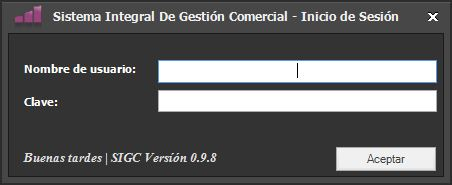
\includegraphics[width=0.70\textwidth]{images/ventanas/ventana-01.jpg}
	\medskip
	\caption{Espacio de trabajo de SIGC.}
\end{figure}
\bigskip


% CAPITULO 1
% Espacio de trabajo
\section{Espacio de trabajo}

Una vez se ha iniciado sesión se abrirá la ventana principal de SIGC, en la que se muestra el espacio de trabajo sobre el cual podrá desenvolverse (\textit{Imagen 1.2}). 
\par
Sobre la parte inferior de la ventana podrá visualizar una barra de estado en la cual se encuentra una opción para cerrar la sesión, la fecha y hora actuales, una opción para acceder al chat provisto por el sistema, información de alertas, UCS, entre otros.
\par
Por otro lado, en la parte superior de la ventana, se encuentra la barra de menú. Dependiendo de los privilegios poseidos por el usuario que ha iniciado sesión se mostrará una cantidad distinta de opciones. Al hacer click en uno de los menús se desplegará otro menú con las distintas opciones permitidas.
\par
El espacio restante, vacío al principio, es en donde se desplegarán las ventanas pertenecientes a las opciones de los menús a los que se accedan.
\bigskip

% Imagen Ventana 02
\begin{figure}[H]
	\centering
	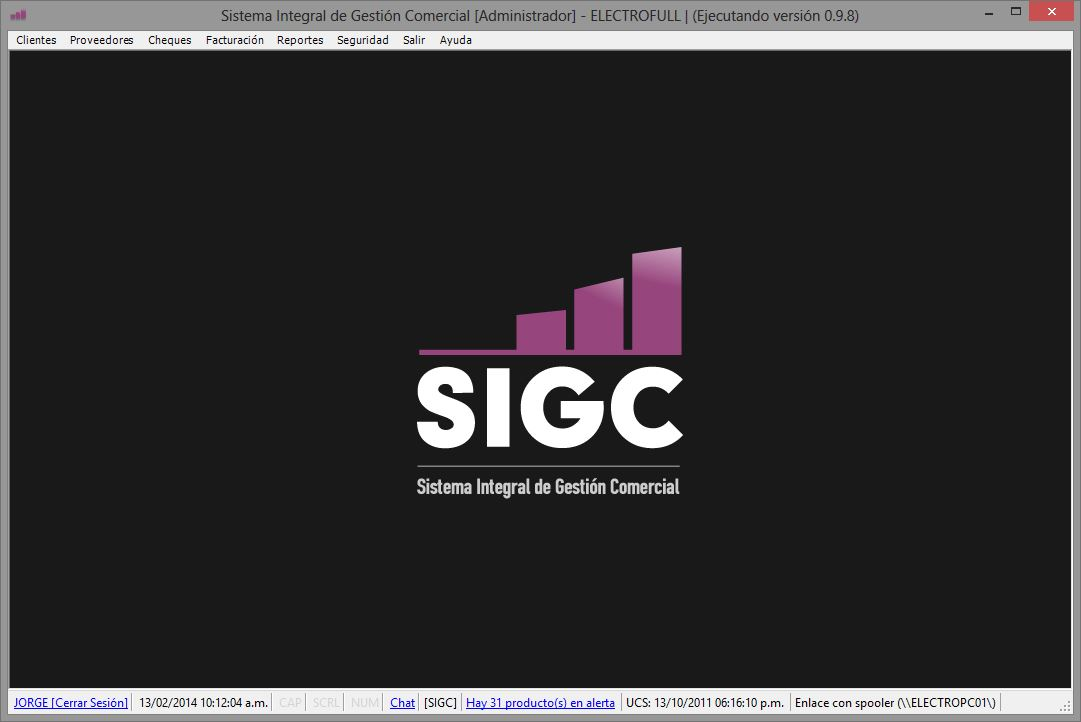
\includegraphics[width=1.0\textwidth]{images/ventanas/ventana-02.jpg}
	\medskip
	\caption{Espacio de trabajo de SIGC.}
\end{figure}
\bigskip



% CAPITULO 1
% Cerrar sesión
\section{Cerrar sesión}

Si desea cambiar de usuario o simplemente cerrar la sesión, siga los siguientes pasos:
\medskip

\begin{enumerate}
	\itemsep=8pt \topsep=0pt \partopsep=0pt \parskip=0pt \parsep=0pt
	
	\item Posiciónese con el puntero del mouse sobre el botón ubicado en el extremo inferior de la ventana que contiene la leyenda \textbf{Usuario [Cerrar Sesión]}, donde en lugar de \textit{Usuario} aparecerá el nombre asociado a su cuenta.

	\item \textbf{Haga click} con el botón izquierdo del mouse.

	\item Sobre el cuadro emergente, donde se le preguntará si se encuentra seguro de finalizar la sesión, \textbf{haga click} en el botón \textbf{Sí}. Recuerde que se cerrarán todas las ventanas activas abiertas en el espacio de trabajo una vez cerrada la sesión.

\end{enumerate}
\medskip

Habiéndose cerrado la sesión aparecerá sobre la ventana principal el formulario de inicio de sesión con el cual podrá volver a ingresar al sistema.
\bigskip



% CAPITULO 1
% Cerrar sesión
\section{Salir del sistema}

Si lo que desea es salir completamente del sistema y finalizar la ejecución de la aplicación, siga los siguientes pasos:
\medskip

\begin{enumerate}
	\itemsep=8pt \topsep=0pt \partopsep=0pt \parskip=0pt \parsep=0pt
	
	\item Diríjase a la barra de menús ubicada en la parte superior de la ventana.

	\item \textbf{Haga click} en la opción \textbf{Salir}.

	\item Sobre el cuadro emergente, donde se le preguntará si se encuentra seguro de salir, \textbf{haga click} en el botón \textbf{Sí}. En este cuadro se le recordará también que debe hacer una copia de seguridad periódicamente.

\end{enumerate}
\medskip




%
% CAPITULO 2
%
\chapter{ABMs}


% CAPITULO 2
% Introducción
\section{Introducción}

En el presente capítulo se introduce al usuario en el uso de formularios ABM. Estos son utilizados para \textit{agregar}, \textit{borrar} y \textit{modificar} los datos que se ingresen en el sistema. 
\par
Dado que SIGC cuenta con varios formularios ABM, se explicará aquí su uso generalizado de manera de que el usuario adquiera conocimiento global de cómo utilizar estos mas allá de las pequeñas diferencias que puedan existir entre unos y otros.
\bigskip\bigskip


% Imagen Ventana 03
\begin{figure}[H]
	\centering
	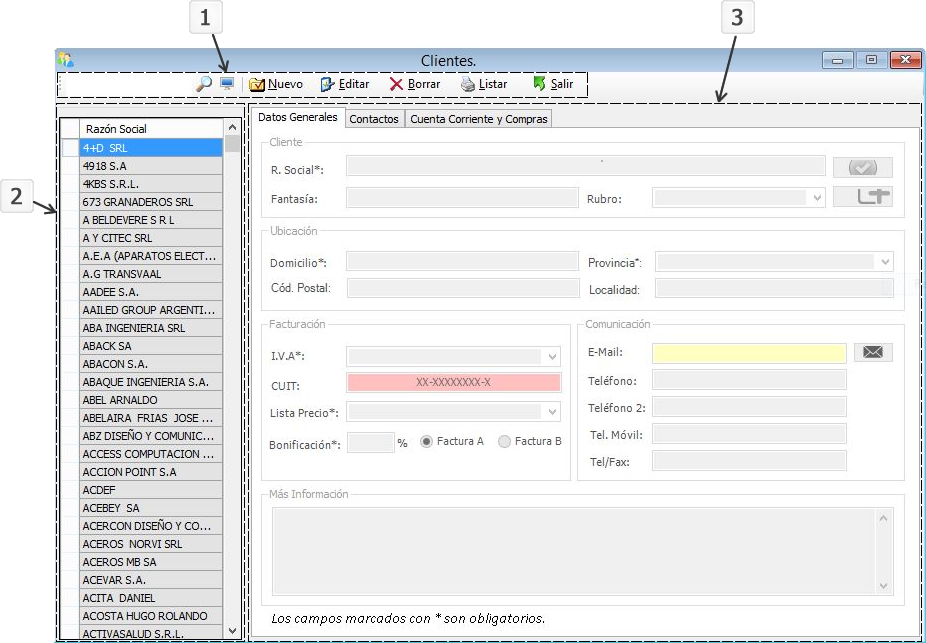
\includegraphics[width=1.0\textwidth]{images/ventanas/ventana-03.jpg}
	\caption{Formulario modelo de un ABM.}
	\medskip
\end{figure}
\bigskip\bigskip
\newpage


Todos los ABM poseen una distribución similar a la que se muestra en la \textit{Imagen 2.1}. Esta se compone de:
\bigskip

\begin{enumerate}
	\itemsep=8pt \topsep=0pt \partopsep=0pt \parskip=0pt \parsep=0pt
	
	\item [] 
\includegraphics[width=0.5cm]{images/number-1.png} \textbf{Menú}: contiene las opciones principales del ABM, entre ellas, \textit{Nuevo} (permite crear un nuevo registro), \textit{Editar} (permite modificar registros existentes), Borrar (permite eliminar un registro existente). A la derecha de la opción \textit{Nuevo} se encuentra un campo que permite filtrar registros escribiendo un patrón de búsqueda y haciendo click sobre la lupa. Junto a esta última se encuentra un botón que al hacerle click proporciona una vista ampliada de los datos;

	\item [] 
\includegraphics[width=0.5cm]{images/number-2.png} \textbf{Listado}: sobre la izquierda se encuentra un listado de todos los registros existentes en ese ABM. Los datos que se muestran son una visión reducida de la totalidad de estos, pudiéndose ampliar tal como se detallo anteriormente;

	\item [] 
\includegraphics[width=0.5cm]{images/number-3.png} \textbf{Campos}: sobre la parte principal de la ventana se encuentran los campos que componen al ABM. Si se presiona el botón \textit{Nuevo} se habilitarán inicializándose vacíos. Una vez completados podrá guardar el nuevo registro haciendo click sobre el botón \textit{Guardar} que aparecerá en el menú superior. En caso de querer volver hacia atrás evitando guardar el registro deberá presionar el botón \textit{Cancelar} ubicado en el mismo menú. Si en lugar de presionar el botón \textit{Nuevo} pulsa la opción \textit{Modificar}, se cargarán en los campos los datos relacionados al registro que se encuentra seleccionado sobre la lista lateral izquierda. Usted podrá así editar dicho registro, y una vez conforme guardar los cambios presionando el botón \textit{Guardar} o deshacer dichas modificaciones pulsando \textit{Cancelar}. Ciertos ABMs pueden contener una amplia cantidad de datos a ingresar, razón por la cual, los campos podrán estar dispuestos en distintas pestañas ubicadas justo debajo de la barra del menú. Al crear un nuevo registro o al modificar uno ya existente usted podrá acceder a la información de cada pestaña haciendo click sobre ella.

\end{enumerate}
\medskip



% CAPITULO 2
% Agregar
\section{Agregar}

Para agregar un nuevo registro o dato en el ABM debe seguir los siguentes pasos:
\medskip

\begin{enumerate}
	\itemsep=8pt \topsep=0pt \partopsep=0pt \parskip=0pt \parsep=0pt
	
	\item Diríjase a la barra de menús ubicada en la parte superior de la ventana.

	\item \textbf{Haga click} en la opción \textbf{Nuevo}. Verá que los campos se habilitarán.

	\item \textbf{Complete} los campos. Recuerde que ciertos ABMs poseen pestañas las cuales contienen campos ordenados según categorías de datos.

	\item Para \textbf{agregar} el registro con los datos ingresados \textbf{haga click} sobre la opción \textbf{Guardar} ubicada en el menú superior. El nuevo registro aparecerá en la lista de la izquierda.

	\item Si en cambio, desea volver hacia atrás y descartar el registro \textbf{haga click} en la opción \textbf{Cancelar}.

\end{enumerate}
\medskip



% CAPITULO 2
% Borrar
\section{Borrar}

Para eliminar un registro existente en el ABM debe seguir los siguientes pasos:
\medskip

\begin{enumerate}
	\itemsep=8pt \topsep=0pt \partopsep=0pt \parskip=0pt \parsep=0pt
	
	\item Diríjase al listado de registros ubicado sobre la parte lateral izquierda de la ventana.

	\item \textbf{Haga doble click} sobre el registro que desee borrar para seleccionarlo. Podrá visualizar sobre los campos la información de dicho registro.

	\item \textbf{Haga click} sobre la opción \textbf{Borrar} ubicada en el menú superior.

	\item Confirme su decisión haciendo \textbf{click} sobre el botón \textbf{Guardar} del menú superior o \textbf{Cancelar} en caso de arrepentirse.

\end{enumerate}
\medskip



% CAPITULO 2
% Modificar
\section{Modificar}


Para modificar un registro existente en el ABM debe seguir los siguientes pasos:
\medskip

\begin{enumerate}
	\itemsep=8pt \topsep=0pt \partopsep=0pt \parskip=0pt \parsep=0pt
	
	\item Diríjase al listado de registros ubicado sobre la parte lateral izquierda de la ventana.

	\item \textbf{Haga doble click} sobre el registro que desee modificar para seleccionarlo. Podrá visualizar sobre los campos la información de dicho registro.

	\item \textbf{Haga click} sobre la opción \textbf{Editar} ubicada en el menú superior. Verá que los campos se habilitarán para su posterior modificación.

	\item Realice las modificaciones que crea necesarias sobre el registro editando los campos.

	\item \textbf{Haga click} sobre la opción \textbf{Guardar} para almacenar los cambios sobre el registro o \textbf{Cancelar} si desea descartar las modificaciones hechas.

\end{enumerate}
\medskip


% CAPITULO 2
% Listar
\section{Listar}

Para crear un reporte con el listado de los registros simplemente debe \textbf{hacer click} sobre la opción \textbf{Listar} ubicada en el menú superior. Se abrirá una ventana la cual muestra el reporte generado. Este podrá ser impreso haciendo click en el ícono que contiene la imagen de una impresora, ubicado en el menú superior de dicha ventana.
\bigskip


% CAPITULO 2
% Filtrar lista de datos
\section{Filtrar lista de datos}

Para filtrar registros existentes en el ABM o para buscar alguno en particular debe seguir los siguientes pasos:
\medskip

\begin{enumerate}
	\itemsep=8pt \topsep=0pt \partopsep=0pt \parskip=0pt \parsep=0pt
	
	\item Diríjase a la barra de menús ubicada en la parte superior de la ventana.

	\item \textbf{Haga click} sobre el campo ubicado en el extremo izquierdo para posicionar allí el cursor.

	\item \textbf{Escriba} la o las palabras con las que desee filtrar o buscar el registro.

	\item \textbf{Haga click} sobre el botón que posee el ícono de una \textbf{lupa}, el cual se encuentra justo al lado del campo sobre el que ha escrito. Verá que sobre el listado ubicado sobre la izquierda aparecerán solo los registros que cumplen con el patrón de búsqueda que se ha ingresado.

	\item Para volver a ver todos los registros posiciónese nuevamente sobre el campo del menú superior y borre su contenido. Luego \textbf{haga click} nuevamente sobre la lupa.

\end{enumerate}
\medskip


% CAPITULO 2
% Ampliar lista de datos
\section{Ampliar lista de datos}

Para ampliar la lista de registros o datos existentes en el ABM debe seguir los siguientes pasos:
\medskip

\begin{enumerate}
	\itemsep=8pt \topsep=0pt \partopsep=0pt \parskip=0pt \parsep=0pt
	
	\item Diríjase a la barra de menús ubicada en la parte superior de la ventana.

	\item \textbf{Haga click} sobre el botón que posee el ícono de un \textbf{monitor}, el cual se encuentra justo al lado del ícono de la lupa.

	\item Podrá ver como se expande el listado de la izquierda para mostrar las demás columnas que componen a los datos relevantes del registro.

	\item Para contraer el listado y volver a la visualización reducida debe \textbf{Presionar} nuevamente el bótón que posee el ícono de un \textbf{monitor}

\end{enumerate}
\medskip


%
% CAPITULO 3
%
\chapter{Clientes}


% CAPITULO 3
% Administrar
\section{Administrar}

Para administrar a los clientes deberá ir al menú superior y \textbf{hacer click} sobre la opción \textbf{Clientes} y luego sobre la opción \textbf{Administrar} del menú contextual que verá desplegado. Se abrirá así la ventana del \textit{ABM de Clientes}. 
\par
Para utilizar el ABM siga los pasos explicados y detallados en el \textit{Capítulo 2}. Podrá ver que el presente ABM cuenta con campos e información separada en tres pestañas:
\smallskip

\begin{itemize}
	\renewcommand{\labelitemi}{\scriptsize\tiny$\blacksquare$} 
	\itemsep=5pt \topsep=0pt \partopsep=0pt \parskip=0pt \parsep=0pt
	
	\item \textit{Datos Generales}: información principal del cliente;

	\item \textit{Contactos}: permite asociar contactos al cliente, como así también modificarlos, eliminarlos o hacerles envíos de emails;

	\item \textit{Cuenta Corriente y Compras}: permite establecer si el cliente cuenta con la modalidad de cuenta corriente, y de ser así, se habilitará la administración general de está (saldo, límite, nivel, asociacion con otras cuentas corrientes y listado de últimas facturas).

\end{itemize}
\medskip


% CAPITULO 3
% Cuenta corriente
\section{Cuenta Corriente}

Para administrar a las cuentas corrientes de los clientes deberá ir al menú superior y \textbf{hacer click} sobre la opción \textbf{Clientes} y luego sobre la opción \textbf{Cuenta Corriente} del menú contextual que verá desplegado. 
\par
La ventana cuenta con un listado de movimientos en su parte central y un detalle del balance en la parte inferior (\textit{Imagen 3.1}). Para administrar una cuenta corriente siga los siguientes pasos:

\begin{enumerate}
	\itemsep=8pt \topsep=0pt \partopsep=0pt \parskip=0pt \parsep=0pt
	
	\item Diríjase y \textbf{haga click} sobre el campo \textbf{Buscar Cliente} para posicionar allí el cursor.

	\item \textbf{Escriba} el nombre de la empresa o parte de esta y presione la tecla \textbf{Enter}. Verá desplegarse una nueva ventana la cual contiene un listado de los clientes que coinciden con lo que se ingresó en el campo de búsqueda.

	\item Busque en la lista el cliente deseado y \textbf{Haga doble click} sobre este mismo para cargar la correspondiente cuenta corriente y comenzar a administrarla. Podrá ver que se cargarán, en caso de existir, una lista de los movimientos realizados hasta el momento.

	\item Para \textbf{agregar} un nuevo movimiento \textbf{haga click} sobre el botón \textbf{Agregar movimiento}.

	\item Para \textbf{modificar} un movimiento existente, \textbf{haga click} sobre un movimiento de la lista para seleccionarlo y luego \textbf{presione} el botón \textbf{Editar movimiento}.

	\item Para \textbf{eliminar} un movimiento existente, \textbf{haga click} sobre un movimiento de la lista para seleccionarlo y luego \textbf{presione} el botón \textbf{Eliminar movimiento}. Se le pedirá que confirme la acción.

	\item Para \textbf{imprimir} el detalle de la cuenta corriente \textbf{haga click} sobre el botón \textbf{Imprimir} ubicado en el extremo superior izquierdo.

\end{enumerate}
\medskip

% Imagen Ventana 06
\begin{figure}[H]
	\centering
	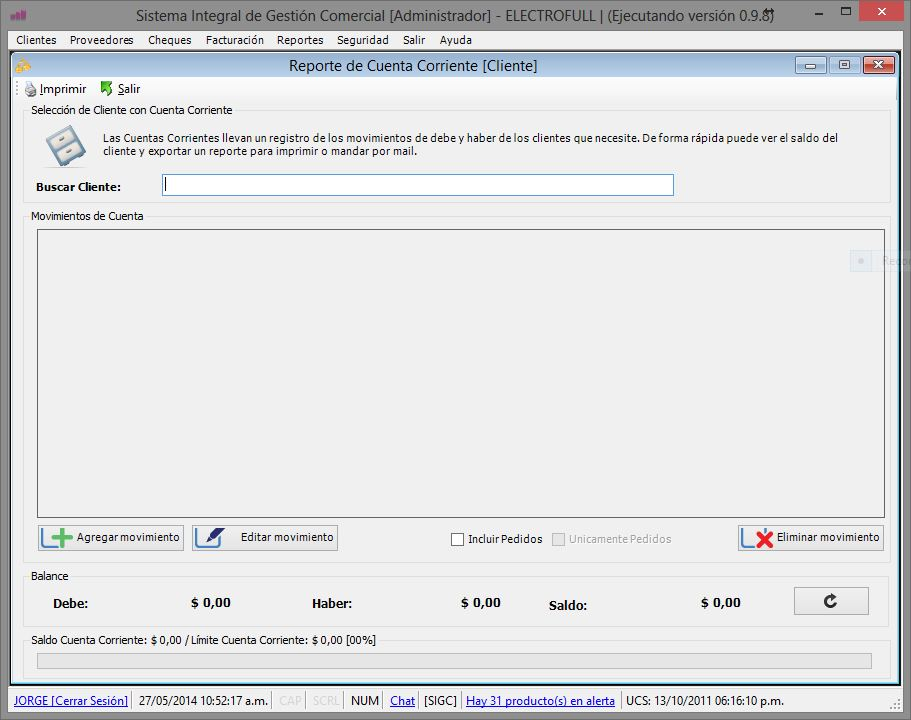
\includegraphics[width=1.0\textwidth]{images/ventanas/ventana-06.jpg}
	\caption{Ventana de administración de cuentas corrientes de clientes.}
	\medskip
\end{figure}
\bigskip



%
% CAPITULO 4
%
\chapter{Proveedores}


% CAPITULO 4
% Administrar
\section{Administrar}

Para administrar los proveedores deberá ir al menú superior y \textbf{hacer click} sobre la opción \textbf{Proveedores} y luego sobre la opción \textbf{Administrar} del menú contextual que verá desplegado. Se abrirá así la ventana del \textit{ABM de Proveedores}. 
\par
Para utilizar el ABM siga los pasos explicados y detallados en el \textit{Capítulo 2}.
\medskip


% CAPITULO 4
% Cuenta corriente
\section{Cuenta Corriente}

Para administrar a las cuentas corrientes de los proveedores deberá ir al menú superior y \textbf{hacer click} sobre la opción \textbf{Proveedores} y luego sobre la opción \textbf{Cuenta Corriente} del menú contextual que verá desplegado. 
\par
La ventana cuenta con un listado de movimientos en su parte central y un detalle del balance en la parte inferior. Para administrar una cuenta corriente siga los siguientes pasos:

\begin{enumerate}
	\itemsep=8pt \topsep=0pt \partopsep=0pt \parskip=0pt \parsep=0pt
	
	\item Diríjase y \textbf{haga click} sobre el campo \textbf{Buscar Proveedor} para posicionar allí el cursor.

	\item \textbf{Escriba} el nombre del proveedor o parte de este y presione la tecla \textbf{Enter}. Verá desplegarse una nueva ventana la cual contiene un listado de los proveedores que coinciden con lo que se ingresó en el campo de búsqueda.

	\item Busque en la lista el proveedor deseado y \textbf{Haga doble click} sobre este mismo para cargar la correspondiente cuenta corriente y comenzar a administrarla. Podrá ver que se cargarán, en caso de existir, una lista de los movimientos realizados hasta el momento.

	\item Para \textbf{agregar} un nuevo movimiento \textbf{haga click} sobre el botón \textbf{Agregar movimiento}.

	\item Para \textbf{modificar} un movimiento existente, \textbf{haga click} sobre un movimiento de la lista para seleccionarlo y luego \textbf{presione} el botón \textbf{Editar movimiento}.

	\item Para \textbf{eliminar} un movimiento existente, \textbf{haga click} sobre un movimiento de la lista para seleccionarlo y luego \textbf{presione} el botón \textbf{Eliminar movimiento}. Se le pedirá que confirme la acción.

	\item Para \textbf{imprimir} el detalle de la cuenta corriente \textbf{haga click} sobre el botón \textbf{Imprimir} ubicado en el extremo superior izquierdo.

\end{enumerate}
\medskip


% CAPITULO 4
% Compras
\section{Compras}

Para administrar las compras que se realizan a los proveedores deberá ir al menú superior y \textbf{hacer click} sobre la opción \textbf{Proveedores} y luego sobre la opción \textbf{Compras} del menú contextual que verá desplegado.
\bigskip


% Imagen Ventana 07
\begin{figure}[H]
	\centering
	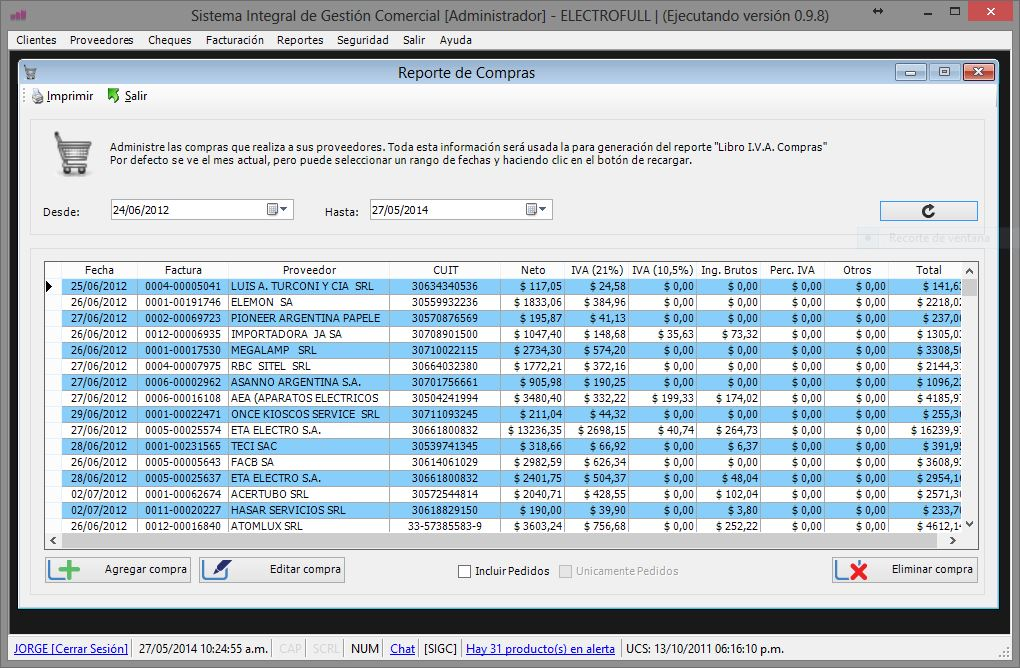
\includegraphics[width=1.0\textwidth]{images/ventanas/ventana-07.jpg}
	\caption{Ventana de administración de compras a proveedores.}
	\medskip
\end{figure}
\medskip


La ventana cuenta con un listado de compras realizadas, las cuales pueden filtrarse de acuerdo a un rango de fechas (\textit{Imagen 4.1}). Para esto seleccione el rango de fechas utilizando los campos \textbf{Desde} y \textbf{Hasta}, y luego presione el botón de actualizacíón ubicado en el extremo opuesto a los campos anteriores. 
\par
Para administrar las compras siga los siguientes pasos:

\begin{enumerate}
	\itemsep=8pt \topsep=0pt \partopsep=0pt \parskip=0pt \parsep=0pt

	\item Para \textbf{agregar} un nuevo movimiento \textbf{haga click} sobre el botón \textbf{Agregar movimiento}.

	\item Para \textbf{modificar} un movimiento existente, \textbf{haga click} sobre un movimiento de la lista para seleccionarlo y luego \textbf{presione} el botón \textbf{Editar movimiento}.

	\item Para \textbf{eliminar} un movimiento existente, \textbf{haga click} sobre un movimiento de la lista para seleccionarlo y luego \textbf{presione} el botón \textbf{Eliminar movimiento}. Se le pedirá que confirme la acción.

	\item Para \textbf{imprimir} el detalle de la cuenta corriente \textbf{haga click} sobre el botón \textbf{Imprimir} ubicado en el extremo superior izquierdo.

\end{enumerate}
\medskip


%
% CAPITULO 5
%
\chapter{Cheques}


% CAPITULO 5
% Administrar
\section{Administrar}

Para administrar los cheques deberá ir al menú superior y \textbf{hacer click} sobre la opción \textbf{Cheques} y luego sobre la opción \textbf{Administrar} del menú contextual que verá desplegado. Se abrirá así la ventana del \textit{ABM de Cheques} (\textit{Imagen 5.1}). 
\par
Para utilizar el ABM siga los pasos explicados y detallados en el \textit{Capítulo 2}. 
\bigskip

% Imagen Ventana 08
\begin{figure}[H]
	\centering
	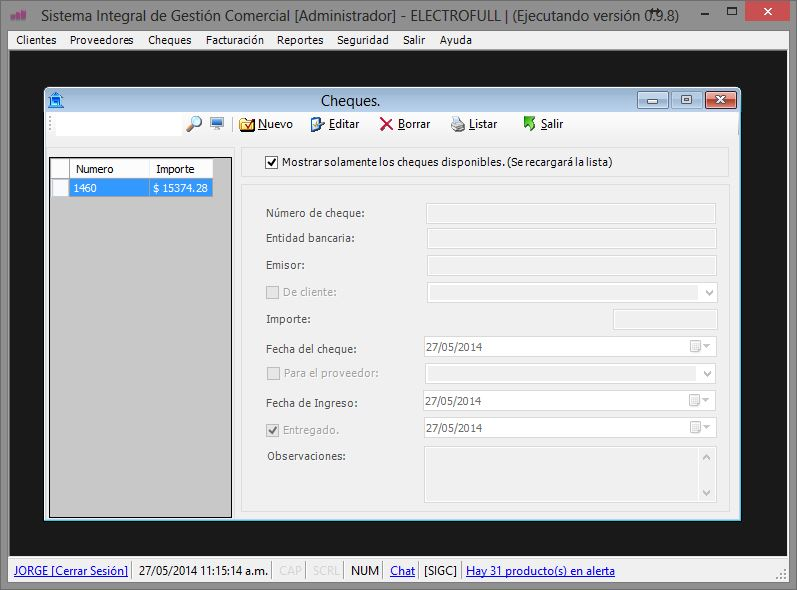
\includegraphics[width=1.0\textwidth]{images/ventanas/ventana-08.jpg}
	\caption{Ventana de administración de cheques.}
	\medskip
\end{figure}
\medskip


%
% CAPITULO 6
%
\chapter{Facturación}


% CAPITULO 6
% Emisiones
\section{Emisiones}

El sistema permite la emisión de distintos tipos de comprobantes, siendo estos los siguientes:

\begin{itemize}
	\renewcommand{\labelitemi}{\scriptsize\tiny$\blacksquare$} 
	\itemsep=3pt \topsep=0pt \partopsep=0pt \parskip=0pt \parsep=0pt
	
	\item Factura
	\item Nota de Crédito
	\item Nota de Débito
	\item Pedido
	\item Devolución
	\item Presupuesto
	\item Recibos

\end{itemize}
\medskip

Para realizar una emisión deberá ir al menú superior, \textbf{hacer click} sobre la opción \textbf{Facturación} y luego sobre la opción \textbf{Emitir}. Seguidamente deberá seleccionar el tipo de emisión que desea. 
\smallskip

% Imagen Ventana 09
\begin{figure}[H]
	\centering
	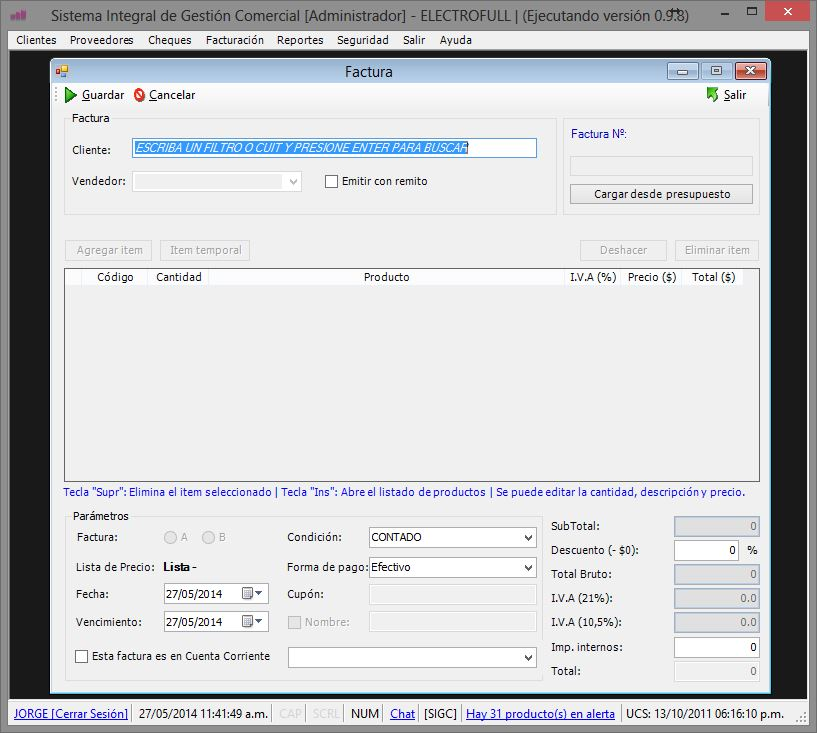
\includegraphics[width=0.63\textwidth]{images/ventanas/ventana-09.jpg}
	\caption{Ventana de emisión de comprobantes.}
	\medskip
\end{figure}
\newpage

Se abrirá una ventana como la que se muestra en la \textit{Imagen 6.1}. Las ventanas de todos los tipos de emisión son similares, razón por la cual solo haremos referencia a la emisión de una Factura. \\
\indent Realice la emisión realizando los siguientes pasos:

\begin{enumerate}
	\itemsep=8pt \topsep=0pt \partopsep=0pt \parskip=0pt \parsep=0pt
	
	\item Diríjase y \textbf{haga click} sobre el campo \textbf{Cliente} para posicionar allí el cursor.

	\item \textbf{Escriba} el nombre del cliente o el CUIT y presione la tecla \textbf{Enter}. Verá desplegarse una nueva ventana la cual contiene un listado de los clientes que coinciden con lo que se ingresó en el campo de búsqueda. \textbf{Haga  doble click} sobre uno de estos para seleccionarlo.

	\item Complete los demás campos relacionados a la factura (Vendedor, N° de Factura, etc.).

	\item \textbf{Haga click} sobre el botón \textbf{Agregar item} o \textbf{Item temporal} para agregar items al comprobante. Los items que agregue se verán en el listado ubicado debajo de dichos botones.

	\item Específique los parámetros del comprobante completando los campos ubicados debajo del listado de items.

	\item \textbf{Haga click} sobre el botón \textbf{Guardar} para guardar el comprobante.

\end{enumerate}
\medskip

Si lo que desea es emitir un recibo, debe ir al menú superior, \textbf{hacer click} sobre la opción \textbf{Facturación} y luego sobre la opción \textbf{Emitir}. Seguidamente deberá ir a \textbf{Recibo} y elegir el tipo de recibo que desea emitir. De esta manera se abrirá una ventana, la cual es similar para todos los tipos de recibo. En la \textit{Imagen 6.2} se muestra una de estas.
\bigskip

% Imagen Ventana 10
\begin{figure}[H]
	\centering
	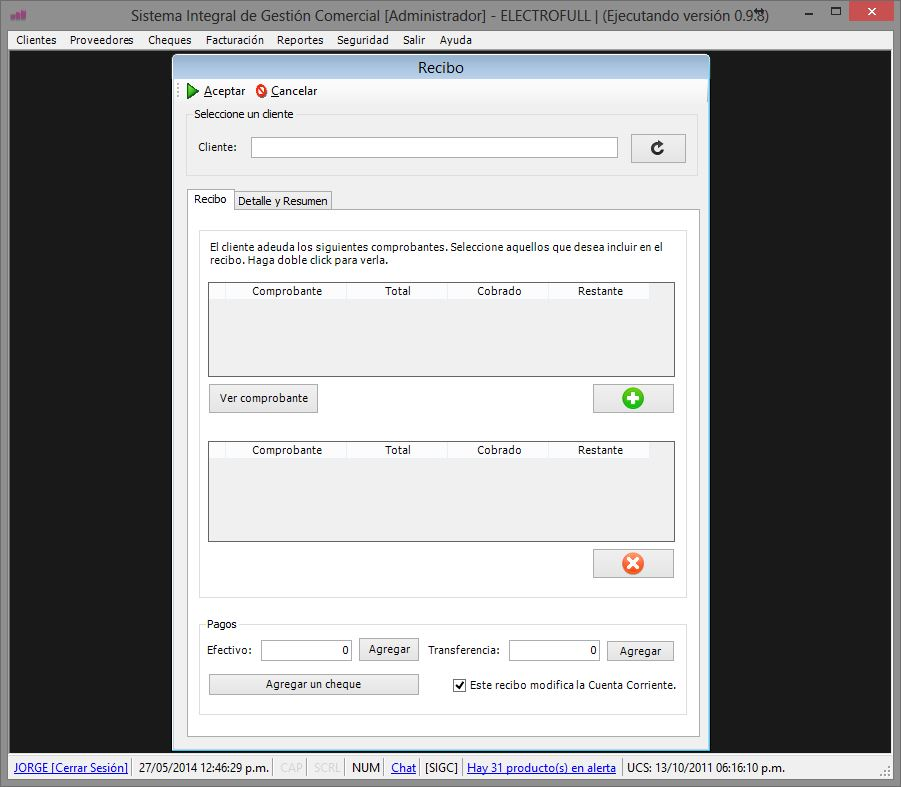
\includegraphics[width=0.80\textwidth]{images/ventanas/ventana-10.jpg}
	\caption{Ventana de emisión de recibos.}
	\medskip
\end{figure}
\bigskip


Para generar un recibo siga los siguientes pasos:

\begin{enumerate}
	\itemsep=8pt \topsep=0pt \partopsep=0pt \parskip=0pt \parsep=0pt
	
	\item Diríjase y \textbf{haga click} sobre el campo \textbf{Cliente} para posicionar allí el cursor.

	\item \textbf{Escriba} el nombre del cliente y presione la tecla \textbf{Enter}. Verá desplegarse una nueva ventana la cual contiene un listado de los clientes que coinciden con lo que se ingresó en el campo de búsqueda. \textbf{Haga  doble click} sobre uno de estos para seleccionarlo.

	\item Elegido el cliente se generará un numero de recibo el cual puede visualizarse sobre la pestaña \textit{Recibo}. Además se cargarán los comprobantes existentes para ese cliente en la primer lista. \textbf{Haga Click} sobre el comprobante que desea agregar al recibo y \textbf{presione} el botón 
\includegraphics[width=0.4cm]{images/agregar.png}. Antes de agregarlos puede ver el comprobante haciendo click sobre el botón \textit{Ver comprobante} ubicado en el extremo inferior de la tabla de comprobantes.

	\item Los comprobantes que agregue al recibo se listaran en la tabla que se encuentra debajo a la tabla de comprobantes existentes. Para quitar comprobantes del recibo \textbf{haga click} sobre este en dicha lista para seleccionarlo y luego \textbf{presione} el botón 
\includegraphics[width=0.4cm]{images/eliminar.png}.

	\item \textbf{Complete} los datos del recibo sobre los campos ubicados en la parte inferior de la pestaña \textbf{Recibo}.

	\item Para ver el detalle y resumen del recibo \textbf{haga click} en la pestaña \textbf{Detalle y Resumen}.

	\item \textbf{Haga click} sobre el botón \textbf{Aceptar} ubicado en el extremo superior izquierdo para \textbf{guardar} el recibo. Se le pedirá que confirme la acción y acto seguido se el consultará si desea \textbf{imprimir} el mismo.

\end{enumerate}
\medskip


% CAPITULO 6
% Gestionar
\section{Gestionar}

Para gestionar los comprobantes \textbf{haga click} sobre la opción \textbf{Facturación} y luego sobre la opción \textbf{Gestionar}. Se abrirá una ventana como la que se muestra en la \textit{Imagen 6.3}.
\smallskip

% Imagen Ventana 11
\begin{figure}[H]
	\centering
	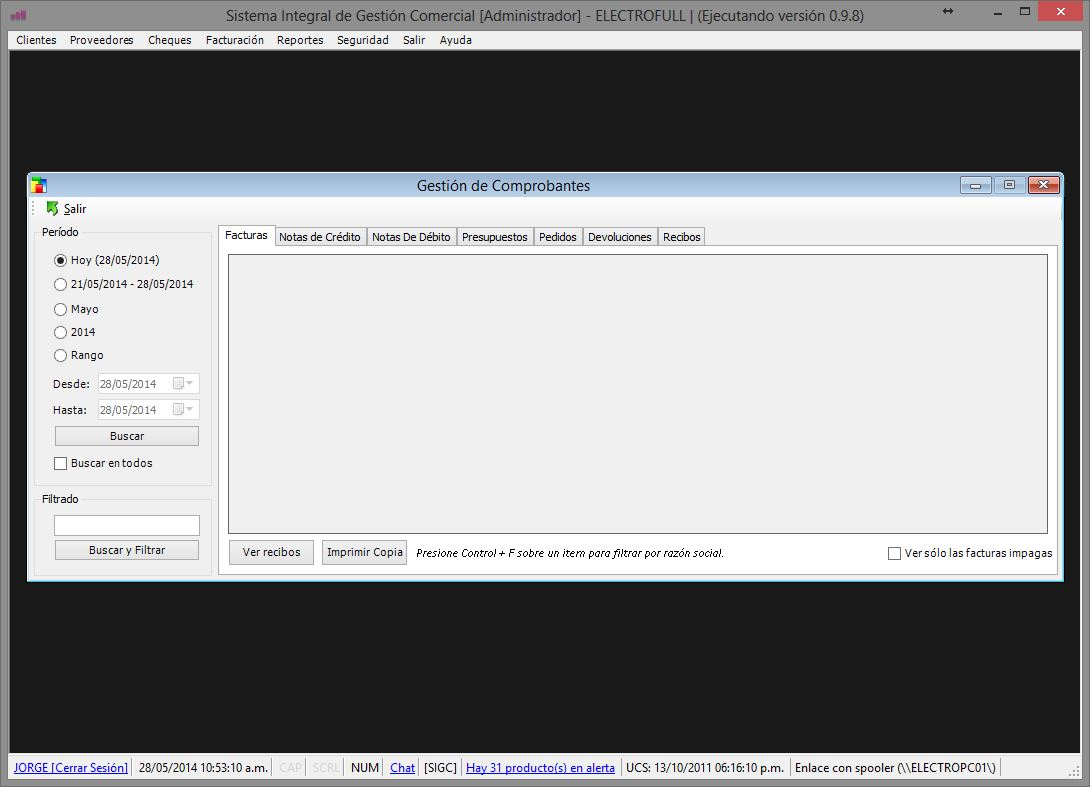
\includegraphics[width=0.79\textwidth]{images/ventanas/ventana-11.jpg}
	\caption{Ventana de Gestion de Comprobantes.}
	\medskip
\end{figure}
\bigskip


Podrá observar una serie de pestañas que clasifican los distintos tipos de comprobantes que existen. Sobre la izquierda se encuentran las opciones que permiten filtrar a estos por fecha o rango de fechas.
\par
Para gestionar los comprobantes siga los siguientes pasos:

\begin{enumerate}
	\itemsep=8pt \topsep=0pt \partopsep=0pt \parskip=0pt \parsep=0pt
	
	\item \textbf{Haga click} sobre la pestaña de la categoría de comprobante que desea visualizar. 

	\item \textbf{Seleccione} el período en las opciones ubicadas en el lado izquierdo de la ventana. Si desea aplicar un rango debe tildar la opción \textbf{Rango} y luego seleccionar las fechas de inicio y fin en los campos que le siguen.

	\item \textbf{Haga click} en el botón \textbf{Buscar} para cargar los comprobantes que cumplen con el filtro aplicado. Tenga en cuenta que solo se cargarán aquellos comprobantes que pertenecen a la pestaña seleccionada. Si desea cargar todos los comprobantes de los diferentes tipos debe tildar antes la opción \textbf{Buscar en todos} ubicada debajo del botón de búsqueda.

	\item Para \textbf{filtrar comprobantes por cliente} diríjase al sector de \textbf{Filtrado} ubicado debajo de los parámetros de búsqueda de comprobantes. \textbf{Haga click} sobre el campo allí ubicado para posicionar el cursor. \textbf{Escriba} el nombre del cliente y presione la tecla \textbf{Enter}. Verá desplegarse una nueva ventana la cual contiene un listado de los clientes que coinciden con lo que se ingresó en el campo de búsqueda. \textbf{Haga  doble click} sobre uno de estos para seleccionarlo. Luego \textbf{haga click} sobre el botón \textbf{Buscar y Filter}.

	\item \textbf{Haga doble click} sobre uno de los comprobantes de la lista para \textbf{abrir} el mismo.

	\item En el caso de las \textbf{Facturas} y los \textbf{Presupuestos} puede imprimir una copia de estos \textbf{haciendo click} sobre el botón \textbf{Imprimir Copia}.

\end{enumerate}
\medskip



% CAPITULO 6
% Reportes
\section{Reportes}

	El sistema permite generar dos tipos de reportes: \textit{Reporte Z} y \textit{Reporte X}. Para esto deberá ir al menú superior y \textbf{hacer click} sobre la opción \textbf{Facturación} y luego sobre la opción \textbf{Reporte Z} o \textbf{Reporte X} del menú contextual que verá desplegado dependiendo de cual se desea imprimir.


%
% CAPITULO 7
%
\chapter{Reportes}


% CAPITULO 7
% Cierre de Caja
\section{Cierre de Caja}

Para visualizar el reporte de \textit{Cierre de Caja} deberá ir al menú superior y \textbf{hacer click} sobre la opción \textbf{Reportes} y luego sobre la opción \textbf{Cierre Caja} del menú contextual que verá desplegado. Se abrirá una ventana como la que se muestra en la \textit{Imagen 7.1}. En esta pueden observarse los detalles de \textit{Ingresos de Caja}, \textit{Vales de Caja}. \textit{Pago a Proveedores} y \textit{Caja} dispuestos en pestañas.
\bigskip

% Imagen Ventana 12
\begin{figure}[H]
	\centering
	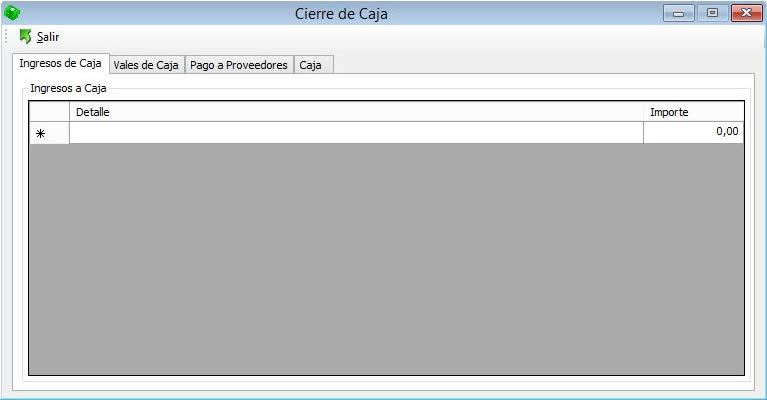
\includegraphics[width=1.0\textwidth]{images/ventanas/ventana-12.jpg}
	\caption{Ventana del reporte de Cierre de Caja.}
	\medskip
\end{figure}
\bigskip


% CAPITULO 7
% Cuenta Corriente
\section{Cuenta Corriente}

Para visualizar el reporte de \textit{Cuentas Corrientes} deberá ir al menú superior y \textbf{hacer click} sobre la opción \textbf{Reportes} y luego sobre la opción \textbf{Cuenta Corriente} del menú contextual que verá desplegado. Se abrirá una ventana como la que se muestra en la \textit{Imagen 7.2}. En ella podrá elegir si desea generar un reporte de \textit{Clientes} o de \textit{Proveedores}, además de poder incluir pedidos tildando la opcion \textit{Incluir Pedidos}. Para imprimir el reporte \textbf{haga click} sobre el botón \textbf{Imprimir}.
\bigskip

% Imagen Ventana 13
\begin{figure}[H]
	\centering
	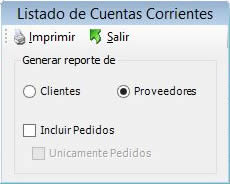
\includegraphics[width=0.4\textwidth]{images/ventanas/ventana-13.jpg}
	\caption{Ventana del reporte de Cuentas Corrientes.}
	\medskip
\end{figure}
\bigskip


% CAPITULO 7
% Libro IVA Compras
\section{Libro IVA Compras}

Para visualizar el reporte de \textit{Libro IVA Compras} deberá ir al menú superior y \textbf{hacer click} sobre la opción \textbf{Reportes} y luego sobre la opción \textbf{Libro IVA Compras} del menú contextual que verá desplegado. Se abrirá una ventana como la que se muestra en la \textit{Imagen 7.3}. En ella deberá elegir el rango de fechas del reporte seleccionando las fechas en los calendarios. Para imprimir el reporte \textbf{haga click} sobre el botón \textbf{Imprimir}.
\bigskip

% Imagen Ventana 14
\begin{figure}[H]
	\centering
	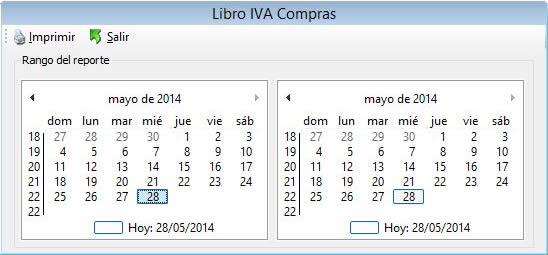
\includegraphics[width=1.0\textwidth]{images/ventanas/ventana-14.jpg}
	\caption{Ventana del reporte de Libro IVA Compras.}
	\medskip
\end{figure}
\bigskip



% CAPITULO 7
% Libro IVA Ventas
\section{Libro IVA Ventas}

Para visualizar el reporte de \textit{Libro IVA Ventas} deberá ir al menú superior y \textbf{hacer click} sobre la opción \textbf{Reportes} y luego sobre la opción \textbf{Libro IVA Ventas} del menú contextual que verá desplegado. Se abrirá una ventana como la que se muestra en la \textit{Imagen 7.4}. En ella deberá elegir el rango de fechas del reporte seleccionando las fechas en los calendarios. Para imprimir el reporte \textbf{haga click} sobre el botón \textbf{Imprimir}.
\bigskip

% Imagen Ventana 15
\begin{figure}[H]
	\centering
	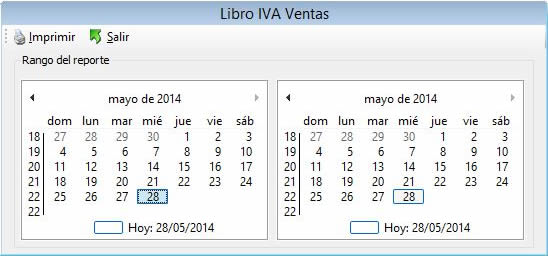
\includegraphics[width=1.0\textwidth]{images/ventanas/ventana-15.jpg}
	\caption{Ventana del reporte de Libro IVA Ventas.}
	\medskip
\end{figure}
\bigskip


% CAPITULO 7
% Productos
\section{Productos}

Para visualizar el reporte de \textit{Productos} deberá ir al menú superior y \textbf{hacer click} sobre la opción \textbf{Reportes} y luego sobre la opción \textbf{Productos} del menú contextual que verá desplegado. Se abrirá una ventana como la que se muestra en la \textit{Imagen 7.5}. En ella podrá elegir si desea generar un reporte de \textit{Todos} o de \textit{Faltantes}, además de poder imprimir el control de inventario tildando la opcion \textit{Imprimir control de Inventario}. Puede también filtrar por proveedor seleccionando a este en el campo \textit{Filtrar por Proveedor}. Para imprimir el reporte \textbf{haga click} sobre el botón \textbf{Imprimir}.
\bigskip\bigskip

% Imagen Ventana 16
\begin{figure}[H]
	\centering
	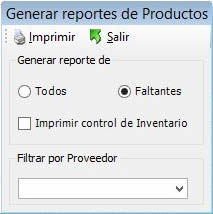
\includegraphics[width=0.4\textwidth]{images/ventanas/ventana-16.jpg}
	\caption{Ventana del reporte de Productos.}
	\medskip
\end{figure}


% CAPITULO 7
% Ventas
\section{Ventas}

Para visualizar el reporte de \textit{Ventas} deberá ir al menú superior y \textbf{hacer click} sobre la opción \textbf{Reportes} y luego sobre la opción \textbf{Ventas} del menú contextual que verá desplegado. Se abrirá una ventana como la que se muestra en la \textit{Imagen 7.6}. En ella podrá elegir si desea generar un reporte de \textit{Hoy}, \textit{Mes corriente} o de \textit{Rango}, además de poder elegir el orden entre \textit{Lo más vendido primero} o \textit{Lo más vendido último}. Otras opciones disponibles son la de incluir pedidos y establecer el rango de fechas. Para imprimir el reporte \textbf{haga click} sobre el botón \textbf{Imprimir}.
\bigskip

% Imagen Ventana 17
\begin{figure}[H]
	\centering
	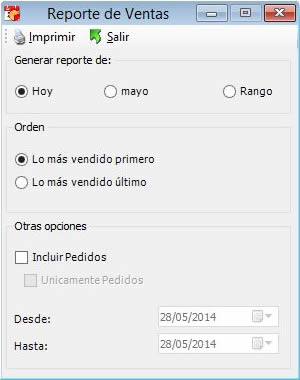
\includegraphics[width=0.4\textwidth]{images/ventanas/ventana-17.jpg}
	\caption{Ventana del reporte de Ventas.}
	\medskip
\end{figure}


% CAPITULO 7
% Cheques
\section{Cheques}

Para visualizar el reporte de \textit{Cheques} deberá ir al menú superior y \textbf{hacer click} sobre la opción \textbf{Reportes} y luego sobre la opción \textbf{Cheques} del menú contextual que verá desplegado. Se abrirá una ventana como la que se muestra en la \textit{Imagen 7.7}. En ella deberá elegir el rango de fechas del reporte seleccionando las fechas en los campos \textit{Desde} y \textit{Hasta}. Puede además incluir los cheques entregados tildando la opcion \textit{Incluir cheques entregados}. Para imprimir el reporte \textbf{haga click} sobre el botón \textbf{Imprimir}.
\bigskip

% Imagen Ventana 18
\begin{figure}[H]
	\centering
	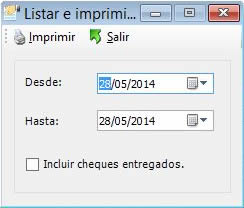
\includegraphics[width=0.36\textwidth]{images/ventanas/ventana-18.jpg}
	\caption{Ventana del reporte de Cheques.}
	\medskip
\end{figure}
\bigskip


%
% CAPITULO 8
%
\chapter{Seguridad}


% CAPITULO 8
% Ajustes
\section{Ajustes}

Para administrar la configuración y preferencias del sistema deberá ir al menú superior y \textbf{hacer click} sobre la opción \textbf{Seguridad} y luego sobre la opción \textbf{Ajustes} del menú contextual que verá desplegado. Se abrirá así la ventana de \textit{Ajustes} (\textit{Imagen 8.1}).
\medskip

% Imagen Ventana 19
\begin{figure}[H]
	\centering
	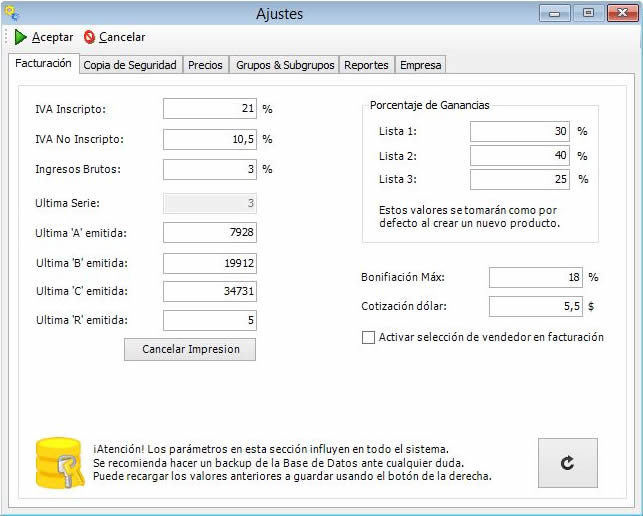
\includegraphics[width=0.8\textwidth]{images/ventanas/ventana-19.jpg}
	\caption{Ventana de Ajustes.}
	\medskip
\end{figure}
\bigskip

En esta podrá ver los distintos tipos de parámetros configurables dispuestos en seis pestañas de acuerdo al tipo de ajuste, siendo estos los siguientes:

\begin{itemize}
	\renewcommand{\labelitemi}{\scriptsize\tiny$\blacksquare$} 
	\itemsep=3pt \topsep=0pt \partopsep=0pt \parskip=0pt \parsep=0pt
	
	\item \textit{Facturación}: permite ajustar los distintos parametros de facturación, tales como el IVA, ingresos brutos, entre otros;
	\item \textit{Copia de Seguridad}: posibilita la realización y gestión de las copias de seguridad del sistema;
	\item \textit{Precios}: administra los precios;
	\item \textit{Grupo \& Subgrupos}: administrar los grupos y subgrupos existentes, como así también la creación de nuevos;
	\item \textit{Reportes}: permite especificar la ruta de la carpeta en donde se alojan los reportes;
	\item \textit{Empresa}: edición de la información general del

\end{itemize}
\medskip


% CAPITULO 8
% Usuarios
\section{Usuarios}

Para administrar a los usuarios del sistema deberá ir al menú superior y \textbf{hacer click} sobre la opción \textbf{Seguridad} y luego sobre la opción \textbf{Usuarios} del menú contextual que verá desplegado. Se abrirá así la ventana del \textit{ABM de Usuarios} (\textit{Imagen 8.2}). 
\par
Para utilizar el ABM siga los pasos explicados y detallados en el \textit{Capítulo 2}. Podrá ver que el presente ABM cuenta con campos e información separada en dos pestañas:
\smallskip

\begin{itemize}
	\renewcommand{\labelitemi}{\scriptsize\tiny$\blacksquare$} 
	\itemsep=5pt \topsep=0pt \partopsep=0pt \parskip=0pt \parsep=0pt
	
	\item \textit{Datos}: información principal del usuario;

	\item \textit{Permisos}: permite establecer que permisos de acceso tiene el usuario sobre el sistema.

\end{itemize}
\smallskip


% Imagen Ventana 20
\begin{figure}[H]
	\centering
	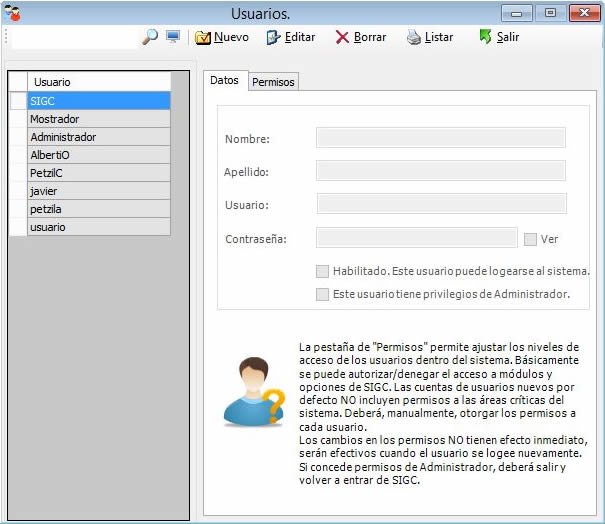
\includegraphics[width=0.8\textwidth]{images/ventanas/ventana-20.jpg}
	\caption{Ventana de Usuarios.}
	\medskip
\end{figure}



% CAPITULO 8
% Vendedores
\section{Vendedores}

Para administrar a los vendedores del sistema deberá ir al menú superior y \textbf{hacer click} sobre la opción \textbf{Seguridad} y luego sobre la opción \textbf{Vendedores} del menú contextual que verá desplegado. Se abrirá así la ventana del \textit{ABM de Usuarios} (\textit{Imagen 8.3}). 
Para utilizar el ABM siga los pasos explicados y detallados en el \textit{Capítulo 2}.
\smallskip
\newpage

% Imagen Ventana 21
\begin{figure}[H]
	\centering
	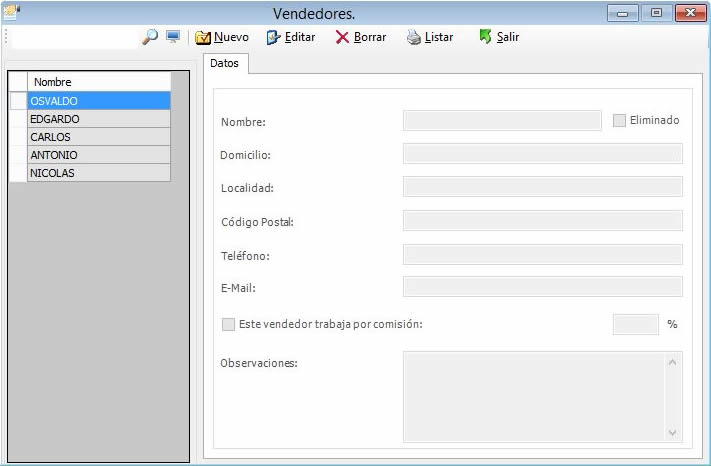
\includegraphics[width=1.0\textwidth]{images/ventanas/ventana-21.jpg}
	\caption{Ventana de Vendedores.}
	\medskip
\end{figure}


% CAPITULO 8
% Comisiones
\section{Comisiones}

Para administrar las comisiones por venta de vendedores del sistema deberá ir al menú superior y \textbf{hacer click} sobre la opción \textbf{Seguridad} y luego sobre la opción \textbf{Comisiones} del menú contextual que verá desplegado. Se abrirá así la ventana de las \textit{Comisiones por venta de vendedores} (\textit{Imagen 8.4}).
\bigskip\bigskip


% Imagen Ventana 22
\begin{figure}[H]
	\centering
	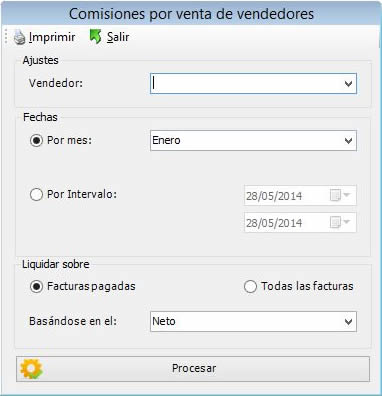
\includegraphics[width=0.5\textwidth]{images/ventanas/ventana-22.jpg}
	\caption{Ventana de Comisiones.}
	\medskip
\end{figure}
\bigskip


Para liquidar las comisiones de un vendedor deberá seguir los siguientes pasos:

\begin{enumerate}
	\itemsep=8pt \topsep=0pt \partopsep=0pt \parskip=0pt \parsep=0pt
	
	\item \textbf{Seleccione} el vendedor sobre el campo \textbf{Vender}.

	\item \textbf{Elija} el período que desea liquidar (por mes o por intervalo).

	\item \textbf{Elija} sobre qué desea liquidar: sobre \textbf{Facturas pagadas} o sobre \textbf{Todas las facturas}.

	\item \textbf{Elija} si desea basarse en el \textbf{Neto} o en el \textbf{Total}.

	\item \textbf{Haga click} en el botón \textbf{Procesar}.

	\item \textbf{Haga click} sobre el botón \textbf{Imprimir} para imprimir el reporte.

\end{enumerate}
\medskip

\newpage
\thispagestyle{empty}

\bigskip\bigskip\bigskip\bigskip

\begin{center}

	
\includegraphics[width=6cm]{images/lupersoft-isotipo-fondo-blanco.png} \\

	\bigskip\bigskip

	\large{Email: info@lupersoft.com} \\
	\large{Teléfono: (+5411) 4862-6569} \\
	\large{Dirección: Soler 4256 - piso 1B (C1425BWV) CABA, Argentina} \\

\end{center}

% {\Huge\fontfamily{pag}\selectfont User Guide \\}
% {\Huge\fontfamily{fvs}\selectfont User Guide \\}
% {\Huge\fontfamily{pbk}\selectfont User Guide \\}
% {\Huge\fontfamily{bch}\selectfont User Guide \\}
% {\Huge\fontfamily{ccr}\selectfont User Guide \\}
% {\Huge\fontfamily{cmr}\selectfont User Guide \\}
% {\Huge\fontfamily{pcr}\selectfont User Guide \\}
% {\Huge\fontfamily{phv}\selectfont User Guide \\}
% {\Huge\fontfamily{fi4}\selectfont User Guide \\}
% {\Huge\fontfamily{lmr}\selectfont User Guide \\}
% {\Huge\fontfamily{LinuxBiolinumT-OsF}\selectfont User Guide \\}
% {\Huge\fontfamily{LinuxLibertineT-OsF}\selectfont User Guide \\}
% {\Huge\fontfamily{pnc}\selectfont User Guide \\}
% {\Huge\fontfamily{ppl}\selectfont User Guide \\}
% {\Huge\fontfamily{ptm}\selectfont User Guide \\}
% {\Huge\fontfamily{uncl}\selectfont User Guide \\}
% {\Huge\fontfamily{put}\selectfont User Guide \\}
% {\Huge\fontfamily{pzc}\selectfont User Guide \\}

\end{document}